
\documentclass[a4paper,oneside,12pt,titlepage]{article}

\usepackage[ngerman]{babel}
\usepackage[utf8]{inputenc}
\usepackage{a4wide}
\usepackage{lmodern}
\usepackage{graphicx}
\usepackage{amsmath}
\usepackage{amsfonts}
\usepackage{eurosym}

\begin{document}
\pagestyle{empty}
\title{Automatisierte Visualisierung\\von meteorologischen Daten}
\author{\\\\\\\\\\\\\\\\\\\\\\Markus Becker\\Swenja Wagner\\Tobias Gerding}

\maketitle
\pagestyle{empty}
\tableofcontents
\thispagestyle{empty}
\pagestyle{plain}
\newpage

% Markus: Bild richtig einfuegen
\begin{figure}
\centering
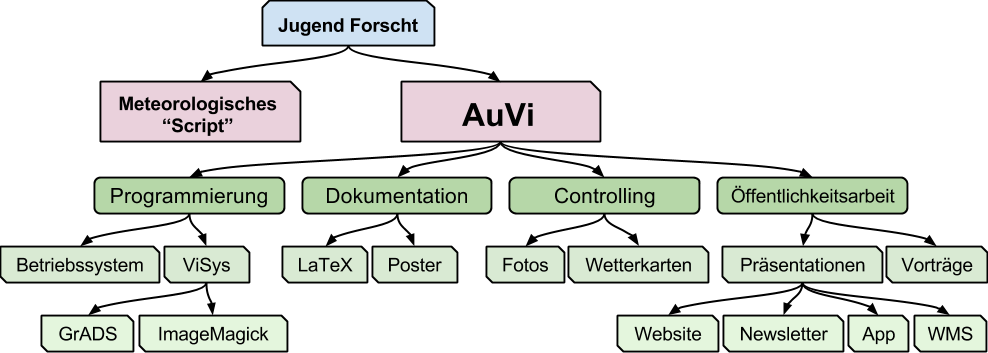
\includegraphics[width=0.9\linewidth]{jfdetails.png} 
\caption{Themengebiete von ''Automatisierte Visualisierung''}
\label{jfdetails}
\end{figure}

Damit Sie sich in diesem Dokument zurecht finden, folgt zunächst ein kurzer Überblick über unsere Projektarbeit Jugend Forscht (Abb. \ref{jfdetails}). Am Schulzentrum Kühlungsborn gibt es zwei Projekte die zu Jugend Forscht gehören. Wir haben zwei Hauptthemen. Eines beschäftigt sich mit den meteorologischen Grundlagen. Die vorliegende Arbeit behandelt aber primär das Projekt AuVi. AuVi steht für Automatisierte Visualisierung von meteorologischen Daten. Das Projekt beinhaltet die Visualisierung von Modellergebnissen, die auf Grundlage meteorologischer Datensätze generiert werden und von uns automatisch als Grafiken verfügbar gemacht werden.\\ Damit wir effektiv an diesem Projekt arbeiten können, haben wir es in vier Aufgabenbereiche eingeteilt: Programmierung, Controlling, wissenschaftliche Dokumentation und Öffentlichkeitsarbeit. Damit etwas automatisiert abläuft, ist zumeist man auf die Hilfe von Computern angewiesen. Wir nutzen Computer auf denen das Betriebssystem Ubuntu (Linux) installiert ist. Auf ihnen entwickeln wir verschiedene Programme, wie zum Beispiel Visys oder UpTexer. Was das für Programme sind, wird später ausführlich erklärt. \\ Der zweite Bereich ist das Controlling. Nachdem verschiedene Prognosen erstellt wurden, müssen diese natürlich überprüft und mit der Realität verglichen werden. Darum geht es in diesem Bereich. Die Arten mit denen man das tun kann sind natürlich zahlreich. Wir konzentrieren uns erst einmal auf den Vergleich mit Bildern und Bodenwetterkarten. \\ Der dritte Teil umfasst die wissenschaftliche Dokumentation. Dabei geht es größtenteils um das Festhalten unserer Fortschritte in Form von Textdokumenten und Postern. Der Text wird mit \LaTeX\mbox{} geschrieben. Das ist eine Makrosprache, die speziel für wissenschaftliche Arbeiten entwickelt wurde. Die Poster gestalten wir mit CorelDraw. Dies wiederum ist ein Programm, das sehr viele Möglichkeiten bietet, um Sachverhalte grafisch darzustellen.\\  
Der vierte und somit letzte Schwerpunkt ist die Öffentlichkeitsarbeit. Dabei geht es um das Publizieren unserer Ergebnisse und Verbreitung von Informationen über unser Projekt. Es beinhaltet die verschiedenen Vorträge und Präsentationen, die wir halten und natürlich auch unseren eigenen Newsletter mit dem wir in der Lage sind, Interessenten auf dem Laufenden zu halten.


\newpage
\section{Vorüberlegung}
    \subsection{Zielstellung}
        Unser Ziel ist die Visualisierung von meteorologischen Daten, die zur Wetterprognose dienen. Die Quelle des geografischen Datensatzes ist das "Global Forecast System". (GFS)\\Wir wollen in der Lage sein für jeden beliebigen Punkt der Erde eine meteorologische Prognose für die kommenden zehn Tage automatisiert zu generieren. Diese Prognosen sollen in Zukunft für Nutzer als Webseite und App zur Verfügung gestellt werden.
    \subsection{Planungsphase}
        Um unsere Ziele zu verwirklichen, entschieden wir ein Linux-System zu nutzen. Auf diesem lassen sich Programme wie zum Beispiel GrADS oder ImageMagick installieren. Auf die Funktionalität dieser Programme sind wir angewiesen, um unsere Ideen umsetzen zu können. Die Verwendungszwecke der eben genannten Programme werden im späteren Teil dieser Arbeit noch näher erläutert. Das meteorologische Wissen vermittelten uns unsere Lehrer und unser Projektleiter Dr. Ronald Eixmann. \\Zudem vergleichen wir unsere Ergebnisse mit den Realdaten. (siehe Projektbereich Controlling) Um unsere Arbeit ausführen zu können, benötigen wir verschiedene Werkzeuge. Damit wir diese verstehen und näher kennen lernen, erarbeiteten wir uns Wissenswertes über diese in einigen Kurzvorträgen.
   
    \subsection{Verbreitungsmöglichkeiten}
        Nach der Fertigstellung unseres Produktes im Rahmen unseres Projektes planen wir es auf möglichst vielen Wegen zu veröffentlichen. Wir orientieren uns hierbei an den vorherrschenden Medien der modernen Gesellschaft. So entschieden wir uns, eine Webseite mit dazugehöriger App zu erstellen. Auf der Webseite soll der Nutzer über sein Konto die Möglichkeit haben, genau die Informationen zu erhalten, die er benötigt. \\Wir sind aber auch für andere Ausgabeformate offen. Eines dieser besonderen Formate ist zum Beispiel das "Weather Monitoring System", kurz WMS. Dieses beinhaltet eine Reihe von Bildschirmen in verschiedenen Hotels, die Wetterinformationen live für die Gäste bereitstellen. \\Eine andere Möglichkeit, die Ergebnisse unseres Projektes publik zu machen, bietet das Präsentieren unserer Ergebnisse in Form von Vorträgen und Präsentationen. Zudem sind viele Geografie-Lehrer an den produzierten Grafiken interessiert. Diese eignen sich sehr gut als Anschauungsmaterial, um den Unterricht interessanter zu gestalten, da sie die aktuellen Gegebenheiten grafisch darstellen. 
    \subsection{Persönlicher Nutzen}
        Einerseits ermöglicht dieses Projekt für uns als Schüler die Arbeit an einem wissenschaftlich komplexen Sachverhalt, andererseits verschafft es uns aber auch Einblicke in den wissenschaftlichen Alltag. Das gibt uns die Chance, uns persönlich mit der Wissenschaft auseinanderzusetzen und erleichtert uns die Antwort auf die Frage, ob wir in Zukunft weiter in diese Richtung gehen wollen. Andererseits bietet es uns die Möglichkeit zu sehen, wie ein kleiner Betrieb sein Einkommen plant und sich selbst verwaltet. 

\section{Umsetzung}
    \subsection{Teilnehmer und ihre Aufgabenbereiche}
        Unser Team besteht aus drei Mitgliedern. Unser jüngstes Mitglied Tobias Gerding geht in die neunte Klasse des Schulzentrums Kühlungsborn. Er ist seit diesem Jahr mit im Team. In seiner Freizeit geht er gerne Segeln, das auch durch das Wetter beeinflusst wird. Seine Aufgabe besteht darin die automatisierten Prognosen an der Wirklichkeit zu überprüfen. Dazu analysiert er unsere Prognosen und vergleicht sie mit selbst gemachten Fotos. Ebenfalls in seinem Aufgabenbereich liegt die Erstellung von Postern, die dann als Anschauungsmaterial in Vorträgen genutzt werden. \\Das nächste Mitglied in unserer Jugend Forscht Gruppe heißt Swenja Wagner und geht in die elfte Klasse. Seit der Gründung unserer Gruppe ist sie mit von der Partie. Swenja ist verantwortlich für die schriftliche Dokumentation und befasst sich auch immer mehr mit den technischen Aspekten unserer Arbeit.\\Markus Becker ist das dritte Mitglied unserer Truppe und befasst sich mit der Programmierung. Er ist wie auch Swenja seit dem Anfang mit dabei. Zusammen bilden sie das Vortrags-Duo.
    \subsection{Methodik und genutzte Mittel}
        Jedes Mitglied teilt seine Zeit selbst ein um an seinen Aufgaben zu arbeiten. Dafür besitzt jeder Schüler einen eigenen Laptop und nutzt je nach seinem Aufgabenbereich verschiedene Programme. Da die Aufgabenbereiche sehr unterschiedlich sind, arbeitet jeder mit anderen Hilfsmitteln. So benutzt z.B. Tobias eher eine Kamera, Stift und Papier. Swenja benutzt LaTeX für die schriftlichen Dokumentation. Das macht sie relativ plattformunabhängig. Markus hingegen programmiert hardware-nah auf einer Linux-Distribution. Er nutzt Programmiersprachen wie Bash, Java und gelegentlich eine FORTRAN ähnliche Scriptsprache für GrADS. Die Emulation des Linux-Betriebssystem erfolgt für alle Mitglieder in einer virtuellen Maschine. \\Da wir nun viele verschiedene Daten auf den unterschiedlichsten Festplatten hatten, drohte es uns den Überblick zu verlieren. Um dies zu vermeiden schrieben wir ein Programm, welches uns das Hoch- und Herunterladen von Daten auf einen gemeinsamen Server vereinfacht. Dort sind unsere Fortschritte nun abgesichert und für jeden Projektteilnehmer frei zugänglich. Dieses Programm vereinfacht den Datenaustausch. So müssen wir zum Beispiel nicht mehr die Daten in E-Mails versenden. 
    \subsection{Arbeitsteilung}
        Damit wir zielorientiert arbeiten, treffen wir uns einmal wöchentlich an einem Dienstag. An diesem Tag besprechen wir unsere Fortschritte und unser weiteres Vorgehen. Falls irgendwelche Anliegen vorliegen, können diese dort geäußert werden. Wir geben Auskunft über unseren bisherigen Stand und führen die Ergebnisse zusammen. Dabei ist besonders wichtig, dass neue Erkenntnisse von allen überprüft und umgesetzt werden. Wenn zum Beispiel Tobias bemerkt hat, dass die Prognosen immer genau zwei Grad daneben liegen, muss der Fehler erst einmal gesucht und dann verbessert werden. Swenja aktualisiert dann gleichzeitig unser Handbuch. Dieses Treffen und unser allgemeiner Arbeitsumgang ist sehr locker, aber es wird dennoch etwas geschafft. Für die Langzeitmotivation ist gerade diese Kombination stark förderlich. 
    \subsection{Kostenkalkulation}
        Bis zum jetzigen Zeitpunkt arbeiten wir mit privaten Mitteln und Ressourcen. Wir haben allerdings angefangen zu überlegen, ob wir die benötigte Rechenleistung auf einem Server bewältigt bekommen. Wenn wir uns diesen Server zulegen würden, könnten wir auch die Webseite darüber betreiben. Die Mindestanforderungen an diesen Server sind: 512 MB RAM, mindestens 20 GB Festplattenspeicher, eine schnelle Internetanbindung (für die Webseite) und eine Domain.\\ Eine Möglichkeit um diese Mindestanforderungen zu erfüllen, bieten V-Server. Diese Kosten circa 70\mbox{ }\euro   \mbox{ }jährlich. Dazu kommt eine Domain, die etwa 15\mbox{ }\euro \mbox{ }im Jahr kostet. Unser Modell sieht vor, Nutzern eine Vielzahl von Paketen anzubieten, welche entweder kostenlos oder kostenpflichtig sind. So kann jeder Nutzer individuell entscheiden wie viel er in die Dienstleistungen investieren möchte, und was er für diese Investition als Gegenleistung bekommt. 

%hb = here, bottom
\begin{figure}[hbp] 
  \centering
     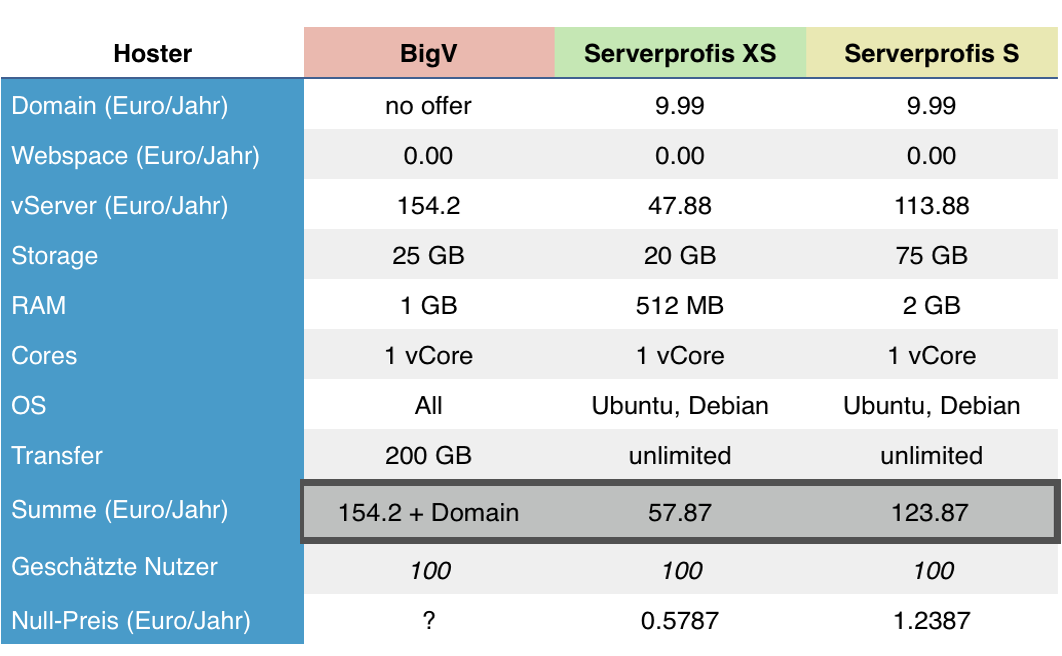
\includegraphics[width=0.8\textwidth]{kostencalc.png}
  \caption{Tabellarische Kostenkalkulation}
\end{figure}

\begin{figure}[hbp] 
  \centering
     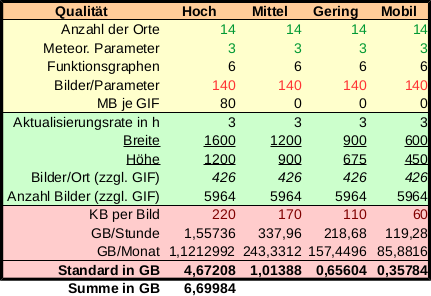
\includegraphics[width=0.8\textwidth]{nutzung.png}
  \caption{Verschiedene Bildqualitäten}
\end{figure}


\newpage
\section{Visys}
\subsection{Visualisierungs System}
        Damit wir unser Ziel erreichen können, entwickelten wir ein eigenes Programm namens Visys, dieses ist die „Exekutive'' von AuVi. AuVi ist der Name unseres Projekts und gleichzeitig eine Abkürzung die für: „Automatisierte Visualisierung von meteorologischen Daten“ steht. Visys ist in Bash geschrieben, das sorgt dafür, dass es sehr schnell ist und auf allen Linux-Distributionen ausführbar ist. Es steht im Mittelpunkt unserer technischen Arbeit. \\Nachdem Visys gestartet wurde, wartet es auf unsere Eingabe. Diese besteht aus gewünschten Orten, mit ihrer dazugehörigen Lage im Gradnetz, die Zeitzone und die zu visualisierenden Parameter, wie zum Beispiel Luftdruck oder Temperatur. Nach dieser Eingabe passt es die bereits existierende Ordnerstruktur je nach gewünschten Ort und Parameter an. \\Wenn zum Beispiel nach dem Ort Rostock mit den Parametern Temperatur und Luftdruck gefragt ist, wird zuerst ein neuer Ordner mit dem Namen „Rostock“ erstellt. Danach werden wiederum in diesem neuen Ordner für jeden einzelnen Parameter neue Ordner erstellt.\\Nach dieser Verwaltungsaufgabe startet Visys mehrmals GrADS, jeweils mit dem gewünschten Ort und Parameter. GrADS übernimmt dann das Herunterladen und die Interpretation der Daten des amerikanischen Wetterdienstes. Anhand des Ortes und des Parameters wählt GrADS dann den richtigen Ordner, in dem es dann die Ergebnisse abspeichert.\\Abschließend ruft Visys ImageMagick auf den nun gefüllten Ordnern auf. ImageMagick übernimmt die Aufbereitung der Grafiken und kombiniert einzelne Grafiken zu Bilderfolgen. In unserem Beispiel hätte GrADS nun seine Ergebnisse in den Ordnern Temperatur und Luftdruck in Form eines Bildes abgespeichert. ImageMagick übernimmt nun Einstellung bezüglich der Auflösung und Qualität und reiht bestimmte Bilder zu einer gif-Datei aneinander. Eine gif-Datei ist ein videoähnliches Format zur Visualisierung der Zeit. In unserem Beispiel würde ImageMagick die Funktionsgrafen für Temperatur und Luftdruck optimieren und eine Übersicht zur gif-Datei zusammenfassen (siehe 5 Visualisierungen).
    

    \subsection{Voraussetzungen}
        \subsubsection{Linux-Distribution}
            Damit unser Programm stabil läuft nutzen wir Ubuntu als Betriebssystem. Das ist ein spezielles System, das auch für das Arbeiten auf Servern ausgelegt ist. Wir nutzen die Programme: GrADS, ImageMagick sowie unsere Eigenentwicklungen.
\newpage
        \subsubsection{Ordnerstruktur}
            Um auf allen Rechnern, die unser AuVi-System benutzen, eine einheitliche Struktur zu garantieren, haben wir uns erlaubt für dieses unter /\$USER/.auvi ein eigenes Verzeichnis zu erstellen. Alle GrADS bezüglichen Daten werden unter /\$USER/.auvi/output abgelegt. Die Standartordner sind input, output, logs und scripts. Diese Ordnerstruktur wird automatisch von unserem Installationsscript Setup.sh, neben der Installation von weiteren benötigten Komponenten, erstellt.
        \subsubsection{Rechenleistung}
            Damit ein Computer fähig ist, unsere Programme auszuführen, benötigt er nicht mehr als 512 MB RAM, einen 32 Bit Prozessor und muss in der Lage sein einen netcdf-Befehl auszuführen. Wir haben für die zu erstellenden Grafiken verschiedene Grundeinstellungen, die Qualität und Größe betreffen. So erzeugen wir HD-Grafiken mit 15 MB pro Durchlauf oder Webformate mit einer deutlich geringeren Auflösung. Die geringere Auflösung der Webformate ist notwendig, damit sie auch schnell auf nicht so leistungsstarken Geräten erscheinen.
        \subsubsection{Modell- und Datenquellen}
            Als Quelle unseres geophysikalischen Datensatzes greifen wir auf die Datenbank des amerikanischen Wetterdienstes zurück. Diese stellen ihre Daten (im Gegensatz zum deutschen Wetterdienst) für jeden frei verfügbar ins Internet. Die Daten für den Wetterdienst werden durch das Global Forecast System (GFS) errechnet. Dieses wurde von den  National Centers for Environmental Prediction entwickelt. Das GFS verbindet verschiedene Datensätze und inter- und extrapoliert die Daten, in Form eines Netzes. Sie benutzen Großrechner um die Daten auf die nächsten zehn Tage herauszurechnen. Die selben Quellen bieten zudem auch Analysedaten an.\\Als zweite Quelle nutzen wir für den Standpunkt Kühlungsborn die schuleigene Wetterstation. Hier überprüft Tobias die gemessenen mit den errechneten Werten. Als meteorologische Parameter werden dort Luftdruck, Temperatur und Niederschlag aufgezeichnet. Um auch die anderen Parameter zu dokumentieren, analysiert er zusätzlich die selbstgemachten Fotos und die generierten Bodenwetterkarten.

        \subsection{Formate der Vorhersage}
            Um die beim amerikanischen Wetterdienst vorliegenden Daten zu interpretieren, nutzen wir ein Programm namens GrADS, welches auch die grundlegende Visualisierung vornimmt. Das oben genannte GFS-Modell errechnet in 1,5 Stunden-Intervallen den Datensatz. Somit haben wir in unserem Programm die Auswahl zwischen den Zeitdaten null und zehn Tagen in 1,5 Stunden Abständen. Natürlich handelt es sich dabei um Modelldaten, die nicht immer genau der Realität entsprechen. Unserer Erfahrung nach hat das GFS-Modell dank seiner Vielzahl an Analysedaten eine hohe Genauigkeit.
    \subsection{Bedienung}
        \subsubsection{Nutzung der Oberfläche}
            Wenn wir auf unseren Linux-Systemen Visys starten, wird uns eine textbasierte Oberfläche angezeigt. In dieser haben wir die Möglichkeit aus einer Vielzahl von Optionen auszuwählen oder schnellstmöglich eine Standard-Routine zu starten. Die Standard-Routine beinhaltet von uns festgelegte Orte und Parameter. Anschließend werden alle Ergebnisse im richtigen Format in einen Webordner kopiert.\\ Zudem können wir wählen, ob wir diese Routine einmalig, n-malig oder permanent ausführen wollen. Dabei wird vom Nutzer erfragt, wie lange Visys zwischen zwei Durchgängen schlafen soll. Schlafen bedeutet in diesem Fall das Warten auf den nächsten Durchgang in Minuten. \\Es gibt allerdings auch Ausnahmen die nach demselben Muster ablaufen, jedoch spezifizierte Orte und Parameter entgegennehmen.

        \subsubsection{Gezielte Wetterprognose}
            Damit Visys alle Informationen hat, die es braucht um eine gezielte Wetterprognose abzugeben, ist es von Nöten, dass ein Nutzer den Ortsnamen, den Breitengrad, den Längengrad, die gewünschte Größe der Übersichtskarte in Grad, die Zeitzone (UTC) und den gewünschten Parameter angibt. Anschließend wird mit allen verfügbaren Daten versucht, eine möglichst lange Prognose zu erstellen. \\Für unser Beispiel Rostock bestände die Befehlszeile aus: dem Ortsnamen Rostock, dem Breitengrad 54.0924406, dem Längengrad 12.0991466, der gewünschten Größe der Übersichtskarte in Grad zum Beispiel 5, der Zeitzone UTC+1, und den gewünschten Parametern Luftdruck und Temperatur.

    \subsection{Fehlerbehebung}
        Leere Prognosen erkennt man daran, dass leere Grafiken erzeugt werden oder das GrADS selbst ein Problem beim Verbinden zum Datenserver meldet. Gründe dafür können sein, dass keine Internetverbindung vorhanden ist, kein Parameter angegeben ist oder ein Punkt, der nicht im Gradnetz der Erde liegt, gewählt wurde.

\newpage
\section{Publikationen}
    \subsection{Webseite}
        Wir planen innerhalb des nächsten Jahres eine Webseite zu kreieren. Diese wird von uns selbst entwickelt und stellt dann das Interface zwischen AuVi und dem Endnutzer dar. Benutzer sollen die Möglichkeit erhalten, nach ihrem Belieben genau die Prognosen zu bekommen, die Sie benötigen. Dafür wird es verschieden komplexe Prognosen geben, um dem Nutzer beim Interpretieren behilflich zu sein. Der Nutzer kann im Hinblick auf Ort und Parameter verschiedene Prognosepakete in seinem Konto an- oder abbestellen. Ein Angler zum Beispiel ist stärker an den Windverhältnissen um den Hafen interessiert und weniger an der Ozonschicht. Ein Forscher interessiert sich möglicherweise genau für diese.\\Zusätzlich wird es zu jeder Prognose einen computergenerierten Text mit Höchsttemperatur, Windgeschwindigkeit und Niederschlagswahrscheinlichkeit geben. So erhoffen wir, uns den interessierten Nutzer auch unterbewusst die Meteorologie nahe zu bringen.\\ Zudem werden wir wirtschaftsorientiert verschiedene Pakete für die interessierten Hotels in und um Kühlungsborn veröffentlichen. Die Prognosen werden dann für den Gast im Foyer zu sehen sein.

    \subsection{App}
        Da in der heutigen Zeit der Marktanteil von Smartphones enorm hoch ist, planen wir zusätzlich eine Version unserer Webseite verpackt in eine iOS oder Android App zu vermarkten. Diese wird reduzierte Grafiken und einen etwas kleineren Funktionsumfang enthalten, damit die Übersicht auf den kleineren Bildschirmen erhalten bleibt. 

    \subsection{Andere Plattformen}
        Ein schon existierendes System ist das „Weather Monitoring System“ (WMS), das in Kühlungsborn verbreitet ist. Auch wenn dort schon Wetterdaten zur Verfügung stehen, sind wir der Meinung, dass unsere Prognosen wegen ihrer Anschaulichkeit auch zusätzlich für die Gäste geeignet sind. Einer dieser Bildschirme hängt zum Beispiel auch im Eingangsbereich unserer Schule, dem Schulzentrum Kühlungsborn.

    \subsection{Öffentlichkeitsarbeit}
        Im Verlaufe unserer Arbeit an diesem Projekt hatten wir schon viele Möglichkeiten unsere Fortschritte und Ideen zu präsentieren. Wir erhielten grundsätzlich eine positive Resonanz. Im Einzelfall wurde auch schon danach gefragt ob man unser System „Beta“-testen kann. Diesem Interesse konnten wir in der Vergangenheit leider noch nicht nachgehen. Aber Interessenten haben die Möglichkeit auf http://www.auvi.tibyte.net, unserer vorübergehenden Domain, den eigens dafür eingerichteten und selbst programmierten Newsletter zu abonnieren.  
        
\section{Zukunft (Neuigkeiten)}
\subsection{Feedback}
Wir besuchten nun die Jugend-forscht Messe in Rostock und stellten unser Projekt vor. Dies war eine perfekte Gelegenheit unsere Routine anzupassen und umzuschreiben und auszutesten, wie sich das Feedback, die Reaktion und die Wirkung auf die Gäste und Zuschauer änderte.\\
Wir entwickelten die oben beschriebene Webseite und machten sie dynamisch. Das heißt, dass je nach gewählten Parametern und Orten auf dem Rechner, der die Ergebnisse generiert eine Website liegt, auf die von aussen zugegriffen werden kann, die immer die aktuellsten Ergebnisse zeigt. Nun ist es eine Leichtigkeit sich ein Netz solcher Computer vorzustellen die ihre Daten zusammenspeisen und eine deutschlandweite Abdeckung bieten.\\ 
Als erstes klares Feedback wollten die Besucher eine klarere Erklärung der gezeigten Grafiken und den Beweis, das die Webseiten, die wir zeigen dynamisch sind. Also schreiben wir an den Tagen, vor und nach den Besuchern und natürlich auch an den Tagen danach an einer vereinfachten Ansicht.
\begin{center}
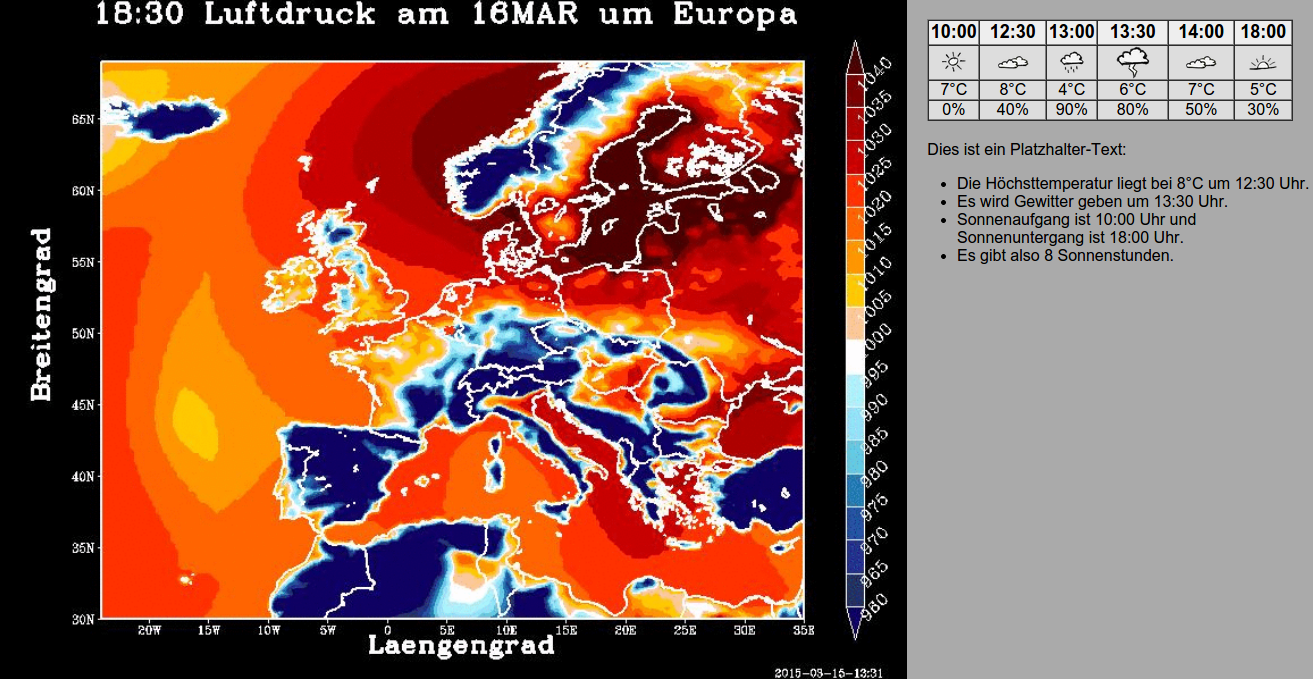
\includegraphics[width=1\linewidth]{display.png} 
\end{center} 
Dies ist ein Prototyp der Anzeige. Diese Anzeige passt sich an den Bilschirm an, läuft immer im Vollbild und zeigt die neusten Ergebnisse, gleich mit Interpretation.\\
Das nächste Feedback das wir erhielten bezog sich auf die Einzigartigkeit und Erreichbarkeit unseres Projektes. Wir führen unsere Routine gerade auf einem Server ein und hoffen in wenigen Wochen unseren Service schon im Internet anbieten können. Unser Service zeichnet sich dadurch aus, das wir zur Laufzeit unseres Angebotes neue Orte und Parameter hinzufügen können und diese mit einer großen Variation präsentieren können. Dies ist eine Neuheit von benutzerdefinierten Wetterprognosen und besonders für den Bereich Tourismus interessant. Außerdem bieten wir somit eine Kombination aus Prognosegrafiken und Prognoseinterpreation an, was auf dem Markt auch eine Seltenheit ist.
\subsection{Weiterentwicklung}
Nach dem Kontakt mit den anderen Jungforschern und dem Austausch über das "Wie" entschieden wir uns unser Projekt von BASH zu Python zu portieren. Unser Skript erfüllt jetzt immernoch die selben Aufgaben, ist aber modularisiert. So können wir in zukunft, wollen wir nur eine bestimmte Subroutine ändern diese ganz leicht auf eine Datei einschränken.\\Desweiteren liegen jetzt alle Informationen über die Orte, Flächen sowie Parameter in JSON Dateien vor, welche mehr und mehr zum Industriestandart werden.
\subsection{Anwendung}
Sobalt die Website und die Anzeigen zuverlässig online sind hält uns nichts auf unsere Ergebnisse auch in Hotels und Ferienwohnungsanlagen sowie der Eingangshalle unserer Schule zu präsentieren. Die Formatierung sowie die Stilisierung ist mit einigen Parametern beim Aufrufen der Webseite übergeben und somit für jeden Anwender angepasst.

%\begin{figure}
%\centering
%\includegraphics[width=0.8\linewidth ,height=0.4\textheight]{Plot11_G_140129_00UT} \
%\caption{globale Temperaturverteilung am 29.01.2014, 0:00 UT, Farbkodierung: blau -5$^{\circ}$C; gr"un 0$^{\circ}$C; orange +5$^{\circ}$C.}
%\end{figure}
%
%\begin{figure}
%\centering
%\includegraphics[width=0.8\linewidth ,height=0.4\textheight]{Plot12_G_140129_12UT} 
%\caption{globale Temperaturverteilung am 30.01.2014, 12:00 UT, Farbkodierung: blau -5$^{\circ}$C; gr"un 0$^{\circ}$C; orange +5$^{\circ}$C.}
%\end{figure}
%\newpage



\newpage
\section{Visualisierungen}
Im Folgenden sehen Sie nun ein paar ausgewählte Beispiele. Das erste Bild auf dieser Seite (links oben) ist ein Konturplot und zeigt die Temperatur in Europa. Breitengrade und Längengrade sind jeweilst links und unten angegeben. Auf der rechten Seite befindet sich eine Legende für die Bedeutung der Farbstufen. Das nächste Bild (rechts oben) ist ein Funktionsgraph und stellt die Parameter Temperatur und Luftdruck in einem sechs tägigen Zeitraum in London dar. Die Skala unten gibt die Zeit an und die Skalen rechts jeweils den Wert in Grad Celcius und Hektopascal.\\
Die verbleibenden zwei Bilder sind ebenfalls Funktionsgraphen für die Temperatur und den Luftdruck. Rechts ist die Prognose für New York und links die für Peking. Diese Orte sind von uns zufällig gewählt und sollen zeigen, dass wir mit Visys jeden beliebigen Ort auf der Erde ansteuern können.\\
Auf der nachfolgenden Seite sind weitere Abbildungen zu erkennen. Die beiden Konturplots in der ersten Reihe zeigen Temperatur (links) und Ozonschicht (rechts) der Welt.
In der zweiten Reihe sind Konturplots Europas zu sehen, die die Parameter Wassersäule (links) und Luftdruck (rechts) veranschaulichen.
Die Funktionsgraphen in der dritten Reihe zeigen die Parameter Temperatur und Luftdruck für Berlin (links) und Temperatur und Wassersäule für Rostock (rechts).\\
Wie schon vorher erwähnt, erzeugen wir auch Videos, die den Verlauf eines Parameters über die Zeit anschaulich darstellen. Da sich diese allerdings nicht auf Papier bringen lassen, haben wir einige Schnappschüsse gemacht und sie in der letzten Reihe zu eine Diaschau zusammengefasst. Der erste Verlauf (oben) zeigt den Luftdruck um Kühlungsborn, der zweite (unten) die Wassersäule.
\begin{center}
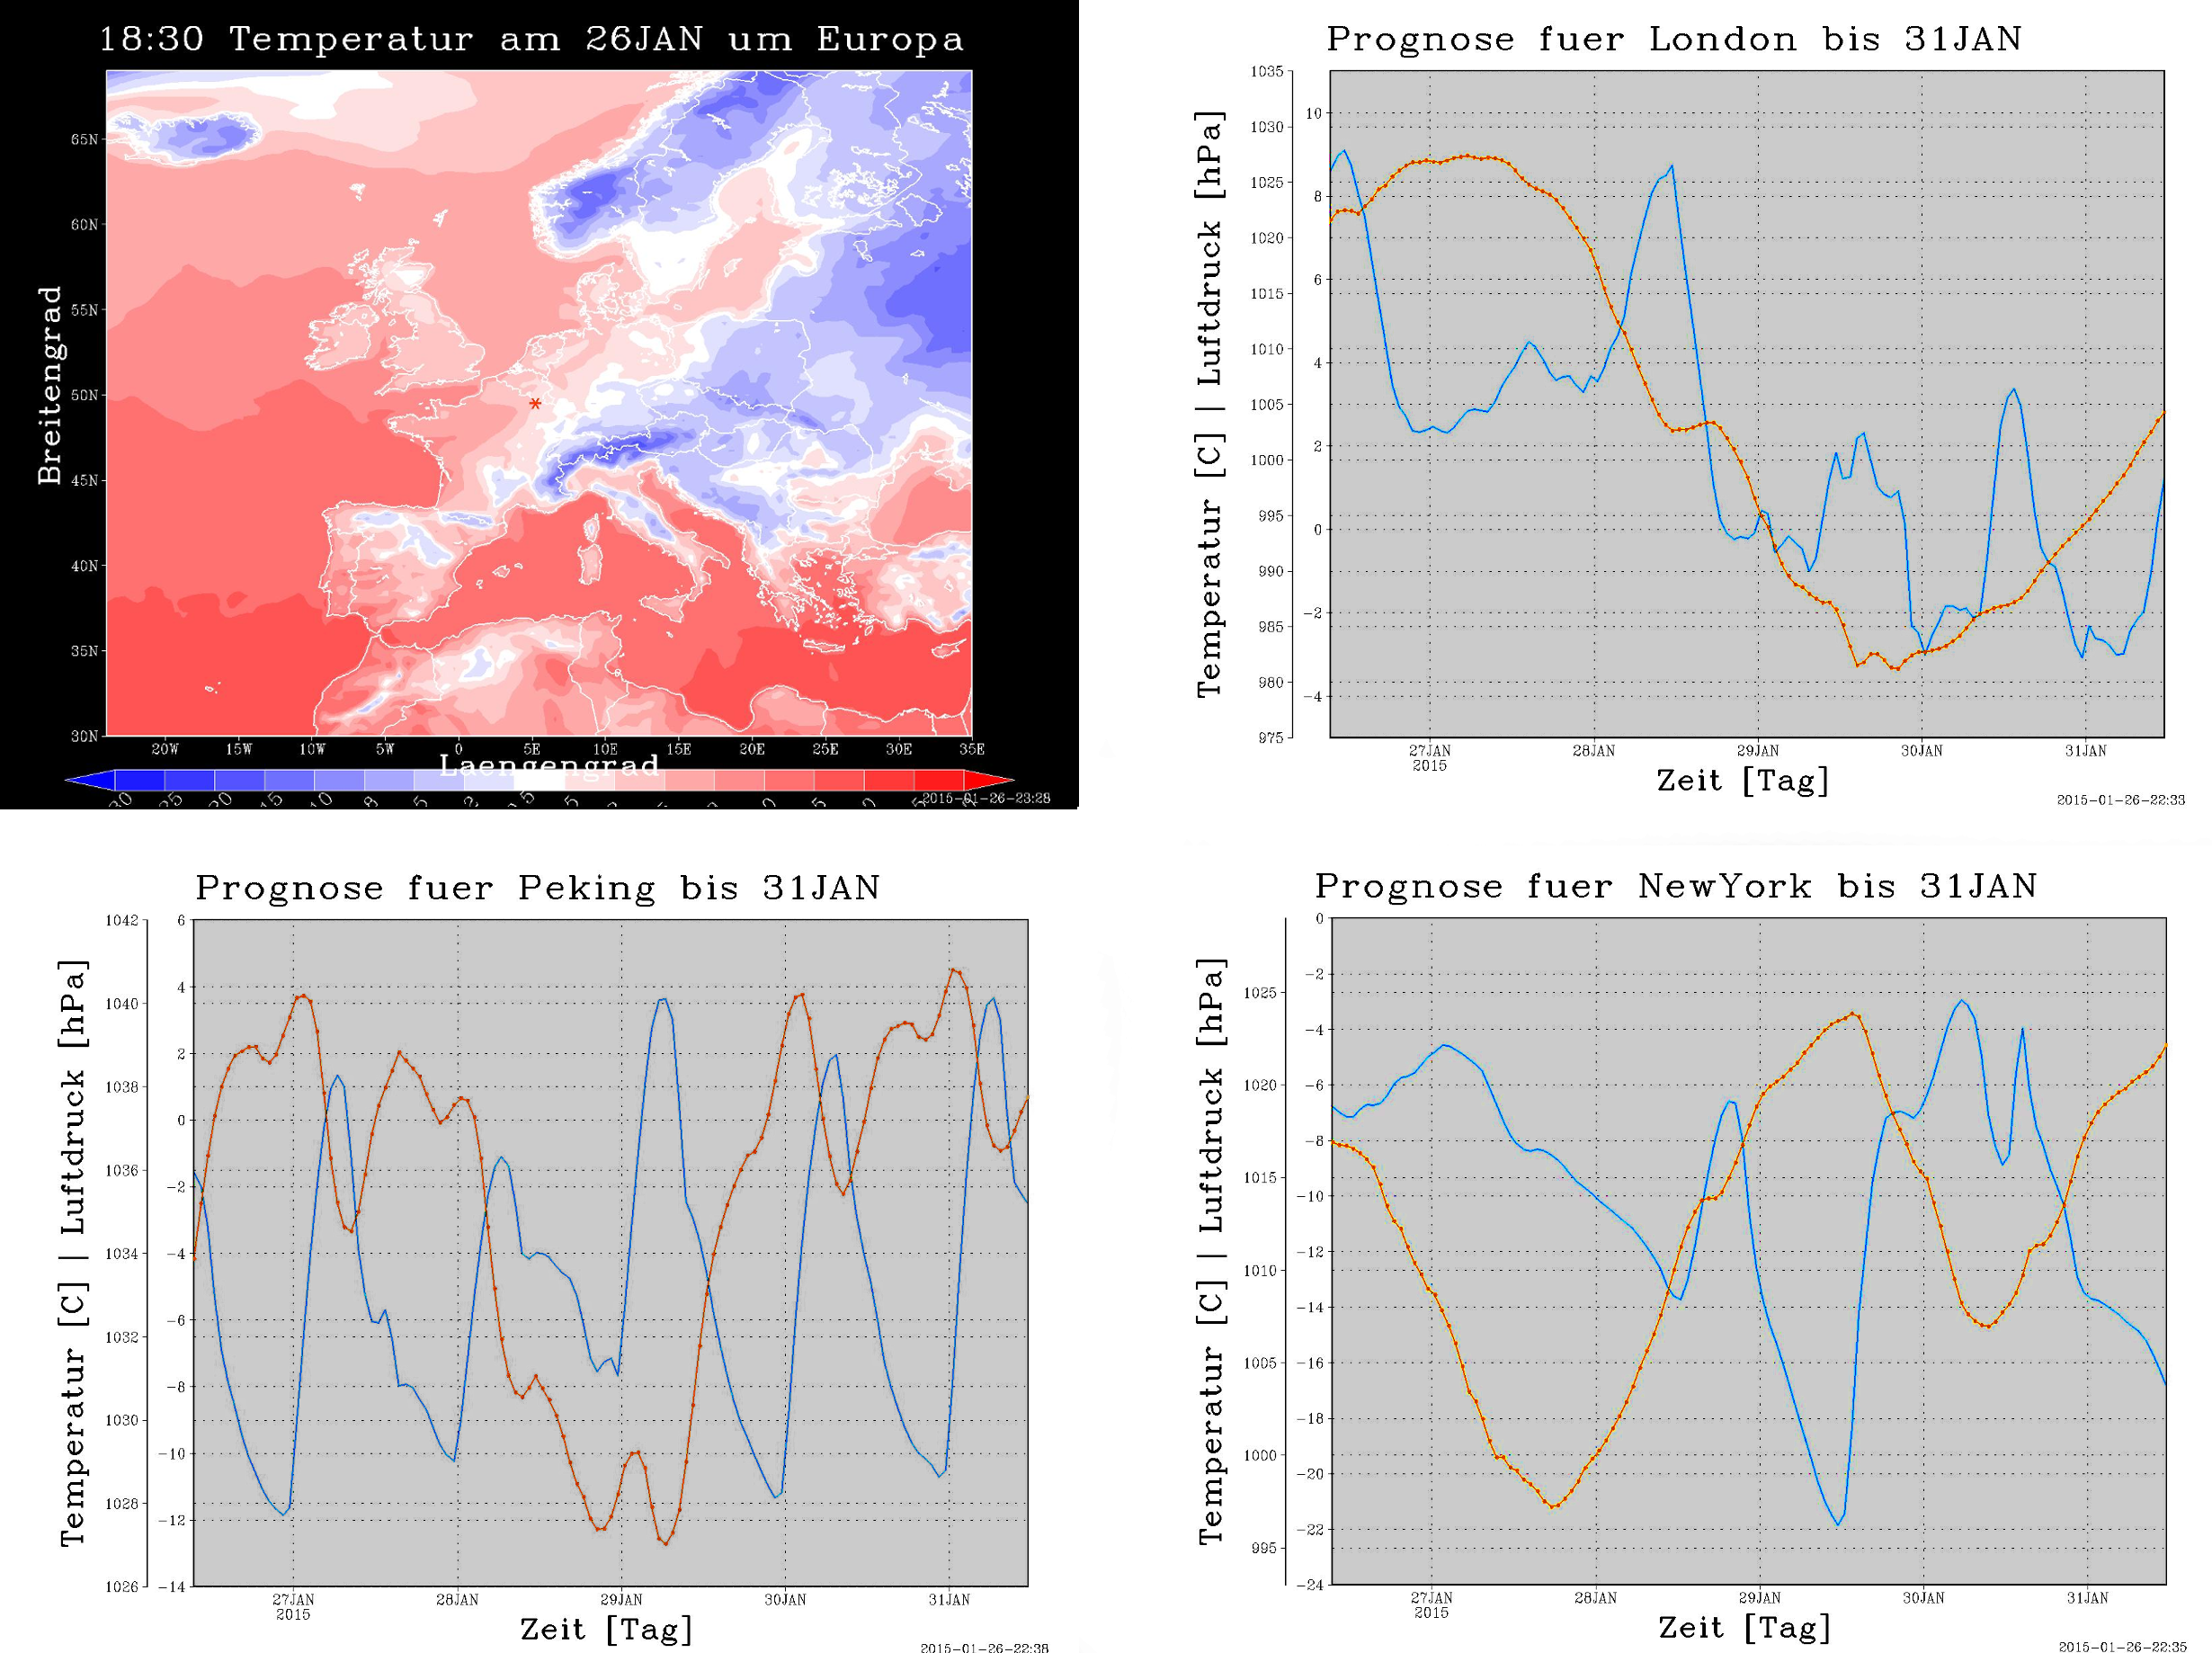
\includegraphics[width=0.9\textwidth, height=0.434\textheight]{vis1.png} 
\end{center}
\newpage
\begin{center}
\includegraphics[width=\textwidth, height=1\textheight]{vis.png} 
\end{center}

\newpage
\Large{Quellen}
\\
\\
\small{
Datenserver \& GFS:\\
http://www.ncdc.noaa.gov/data-access/model-data/model-datasets/global-forcast-system-gfs \\(13.01.2015)\\\\
Kühlungsborner Seewetterstation:\\
http://seewetterstation-kborn.de/ \\(15.01.2015)\\\\
GrADS-Website:\\
http://iges.org/grads/ \\(15.01.2015)\\\\
Imagemagick:\\
http://www.imagemagick.org/ \\(15.01.2015)\\
}



\newpage
\Large{Selbstständigkeitserklärung}\\
\\
\small Hiermit erklären wir, dass wir die vorliegende Arbeit selbständig angefertigt, nicht anderweitig zu Prüfungszwecken vorgelegt und keine anderen, als die angegebenen Hilfsmittel verwendet haben. Zudem waren alle verwiesenen Webseiten zum Zeitpunkt der Linksetzung gültig und erreichbar. Wörtlich und sinngemäße Übernahmen aus anderen Werken sind als solche gekennzeichnet.
\\ 



\end{document} 
